% =============================================================================
% 3. IMPLEMENTACION
% =============================================================================
\section{Implementaci\'on}
\label{sec:implementation}

\subsection{API REST con FastAPI}

La API expone dos endpoints principales:

\begin{itemize}
    \item \texttt{GET /health}: verificaci\'on de estado del servicio.
    \item \texttt{POST /predict}: clasificaci\'on de radiograf\'ia de t\'orax (acepta JPEG/PNG, m\'aximo 10MB).
\end{itemize}

El ciclo de vida de la aplicaci\'on gestiona la carga del modelo ONNX al iniciar y su liberaci\'on al apagar:

\begin{lstlisting}[language=Python, caption={Lifespan del modelo ONNX en FastAPI.}]
@asynccontextmanager
async def lifespan(app: FastAPI):
    settings: Settings = app.state.settings
    try:
        app.state.inference_service = InferenceService(
            settings.model_path
        )
    except FileNotFoundError as exc:
        raise SystemExit(1) from exc
    yield
    app.state.inference_service.close()
\end{lstlisting}

\subsection{Servicio de inferencia}

El modelo se carga una sola vez al arrancar y se reutiliza para todas las solicitudes:

\begin{lstlisting}[language=Python, caption={InferenceService con ONNX Runtime.}]
class InferenceService:
    def __init__(self, model_path: str) -> None:
        path = Path(model_path)
        if not path.is_file():
            raise FileNotFoundError(f"Model not found: {model_path}")
        self.session = ort.InferenceSession(model_path)

    def predict(self, tensor: NDArray[np.float32]):
        results = self.session.run(
            ["predictions"], {"image": tensor}
        )
        return results[0][0]  # 5 probabilidades
\end{lstlisting}

La entrada es un tensor float32 de forma $(1, 1, 224, 224)$ con valores de p\'ixel en $[0, 255]$. El modelo maneja la normalizaci\'on internamente (normalizaci\'on embebida en ONNX), eliminando el riesgo de training-serving skew.

\begin{figure}[H]
    \centering
    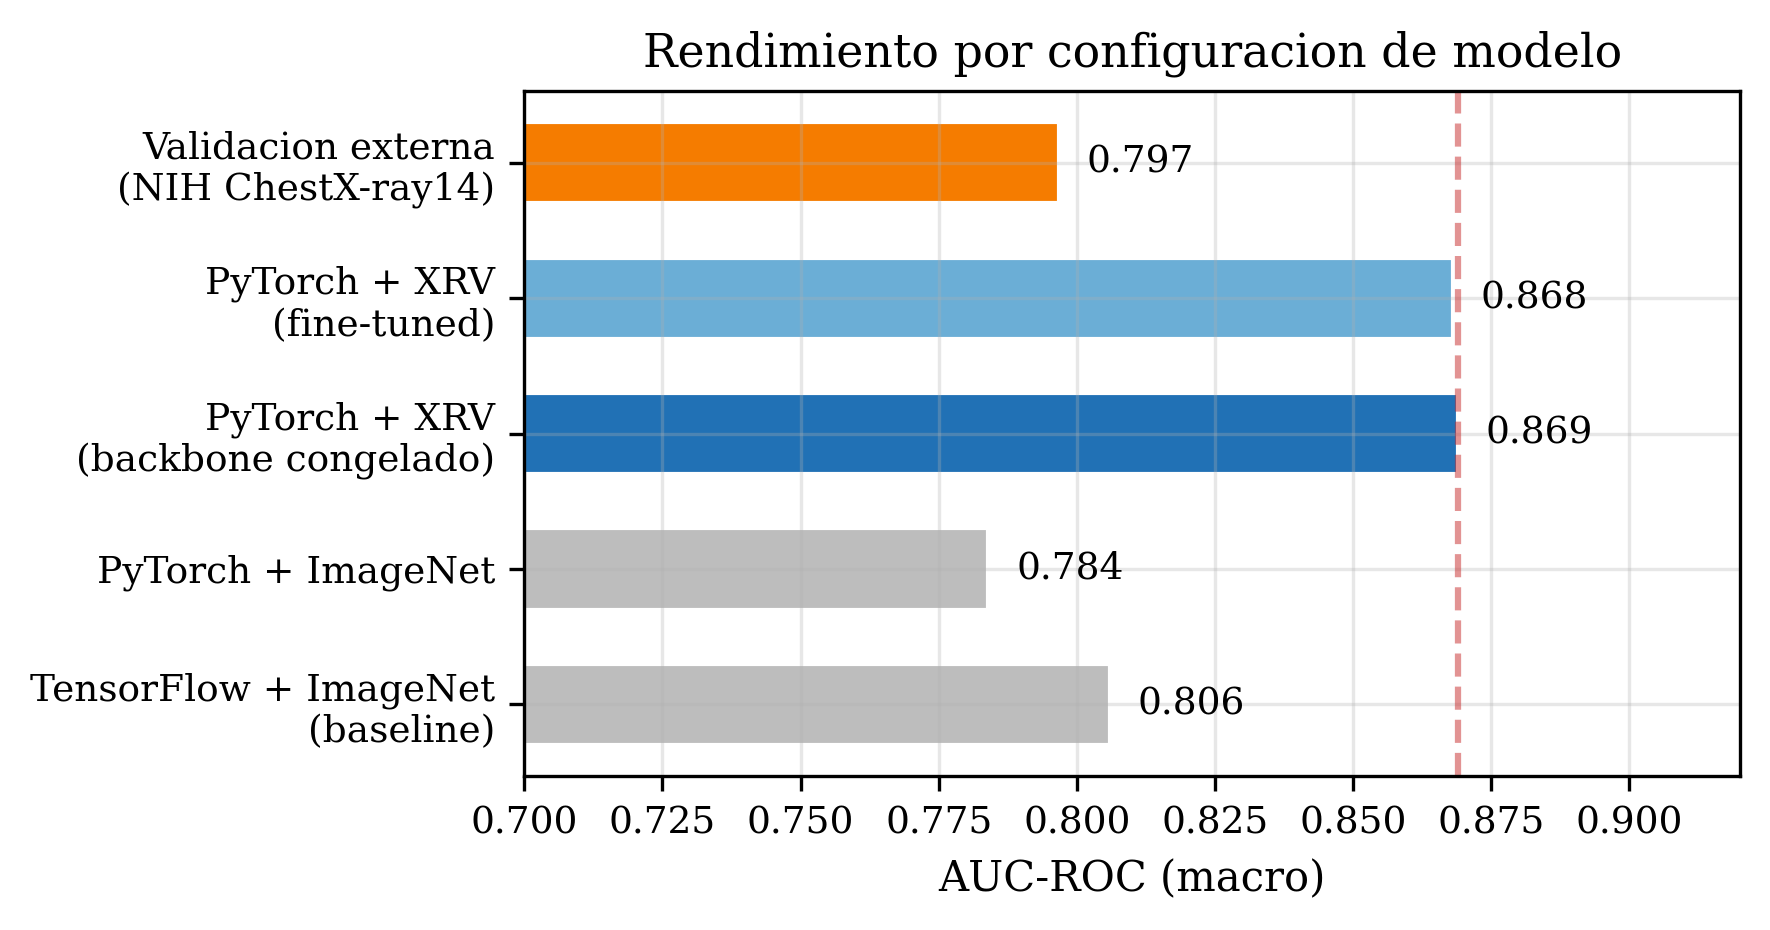
\includegraphics[width=0.85\textwidth]{figures/auc-roc-model-configs.png}
    \caption{Curvas AUC-ROC por patolog\'ia del modelo DenseNet121 + TorchXRayVision. AUC macro = 0.869.}
    \label{fig:auc-roc}
\end{figure}

\subsection{Dockerfile multi-stage}

El Dockerfile aplica las mejores pr\'acticas de producci\'on vigentes en 2026:

\begin{lstlisting}[language={}, caption={Dockerfile multi-stage (simplificado).}]
# Stage 1: Build
FROM python:3.14-slim-bookworm AS builder
COPY --from=ghcr.io/astral-sh/uv:0.11.21 /uv /bin/
ENV UV_COMPILE_BYTECODE=1
ENV UV_LINK_MODE=copy
WORKDIR /build
COPY pyproject.toml uv.lock ./
RUN uv sync --frozen --no-dev --no-install-project
COPY app/ ./app/
RUN uv sync --frozen --no-dev --no-editable

# Stage 2: Runtime
FROM python:3.14-slim-bookworm AS runtime
RUN groupadd -r chest-xpert && useradd -r -g chest-xpert ...
COPY --from=builder --chown=chest-xpert:chest-xpert \
    /build/.venv /app/.venv
COPY --chown=chest-xpert:chest-xpert models/ ./models/
USER chest-xpert
HEALTHCHECK CMD ["python", "-c", "...urlopen(health)..."]
CMD ["python", "-m", "uvicorn", "app.main:app", ...]
\end{lstlisting}

\noindent
Pr\'acticas aplicadas en el Dockerfile:

\begin{itemize}
    \item \textbf{Multi-stage build}: separa dependencias de compilaci\'on del runtime final.
    \item \textbf{UV pinned} (v0.11.21): resoluci\'on r\'apida y determinista de dependencias.
    \item \textbf{Bytecode precompilado} (\texttt{UV\_COMPILE\_BYTECODE=1}): startup m\'as r\'apido.
    \item \textbf{Cache mounts}: builds incrementales eficientes en CI.
    \item \textbf{Intermediate layers}: dependencias y c\'odigo en capas separadas para cache \'optima.
    \item \textbf{Non-root user}: principio de m\'inimo privilegio.
    \item \textbf{Modelo embebido}: no requiere vol\'umenes para arrancar.
    \item \textbf{OCI Labels}: metadata para trazabilidad con \texttt{docker inspect}.
    \item \textbf{HEALTHCHECK}: integraci\'on con orquestadores (Docker, ECS, Kubernetes).
\end{itemize}

\subsection{Gesti\'on de configuraci\'on}

La configuraci\'on se maneja con \texttt{pydantic-settings}, cargando valores desde variables de entorno con prefijo \texttt{CHEST\_XPERT\_}:

\begin{table}[H]
\centering
\caption{Variables de configuraci\'on del servicio.}
\small
\begin{tabular}{llp{5cm}}
\toprule
\textbf{Variable} & \textbf{Default} & \textbf{Descripci\'on} \\
\midrule
\texttt{MODEL\_PATH} & \texttt{models/...onnx} & Ruta al modelo ONNX \\
\texttt{SERVER\_PORT} & 8000 & Puerto del servidor \\
\texttt{RGB\_DIFF\_THRESHOLD} & 5.0 & Umbral del filtro de seguridad \\
\texttt{CORS\_ORIGINS} & localhost:4200 & Or\'igenes CORS permitidos \\
\bottomrule
\end{tabular}
\end{table}

Nunca se incluyen secretos dentro de la imagen. Las API keys se inyectan en runtime mediante \texttt{-e} o archivos \texttt{.env} montados.
